\documentclass[11pt]{article}
\usepackage[utf8]{inputenc}
\usepackage{graphicx}
\usepackage{caption}
\usepackage{amsmath}
\usepackage{geometry}
\geometry{margin=1in}

\title{Quantum-Enhanced Active Learning for Accelerated Materials Discovery}
\author{Arnav Kapoor \\
Indian Institute of Science Education and Research, Bhopal \\
\texttt{arnavkapoor23@iiserb.ac.in}}
\date{}

\begin{document}
\maketitle

\begin{abstract}
This extended abstract presents a quantum-inspired active learning framework that encodes candidate materials as amplitude-style states and aggregates multi-observable uncertainty to prioritize experiments. The method computes per-candidate observable variances and symmetric cross-observable covariances (electronic, structural, thermodynamic) and combines them into a single selection score $U_{\mathrm{total}}$ that captures correlated sources of uncertainty. The selection rule is model-agnostic and computationally tractable on classical hardware. Experiments on band gap and formation-energy regression (five trials, nine baselines) show improved sample efficiency (roughly 25–35% reduction in experimental budget) and higher final $R^2$ (band gap: $0.847 \pm 0.023$; formation energy: $0.792 \pm 0.031$), with paired t-tests reporting $p<0.01$ against top baselines. Code and preprocessing scripts are provided for reproducibility.
\end{abstract}

\section*{Introduction}
Discovering materials with target properties is often limited by expensive experiments or high-fidelity simulations. Active learning reduces cost by choosing experiments expected to be maximally informative, but classical uncertainty measures can miss coupled, multi-physical phenomena. We propose a quantum-inspired representation and a multi-observable uncertainty aggregation that explicitly models cross-observable covariance, producing a richer uncertainty signal for selection.

\section*{Method}
Each candidate material is represented by a normalized feature vector mapped to an amplitude representation $|\psi\rangle=\sum_j \alpha_j |f_j\rangle$. We define observables $\{\hat{O}_k\}$ corresponding to physical domains (e.g., electronic, structural, thermodynamic). For a state $|\psi\rangle$ the variance and symmetric covariance are
\begin{align}
\sigma^2(\hat{O}_k) &= \langle\psi|\hat{O}_k^2|\psi\rangle - \langle\psi|\hat{O}_k|\psi\rangle^2,\\
\mathrm{Cov}(\hat{O}_k,\hat{O}_l) &= \langle\psi|\tfrac{\hat{O}_k\hat{O}_l+\hat{O}_l\hat{O}_k}{2}|\psi\rangle - \langle\psi|\hat{O}_k|\psi\rangle\langle\psi|\hat{O}_l|\psi\rangle.
\end{align}
The aggregate selection score is
\[ U_{\mathrm{total}} = \sqrt{\sum_k |\alpha_k|^2 \sigma^2(\hat{O}_k) + \sum_{k\neq l} \alpha_k^*\alpha_l\,\mathrm{Cov}(\hat{O}_k,\hat{O}_l)}. \]
Operators are implemented as structured (sparse/low-rank) matrices; expectations and covariances are evaluated via matrix–vector products, keeping complexity practical for pools of thousands.

\begin{figure}[ht]
\centering
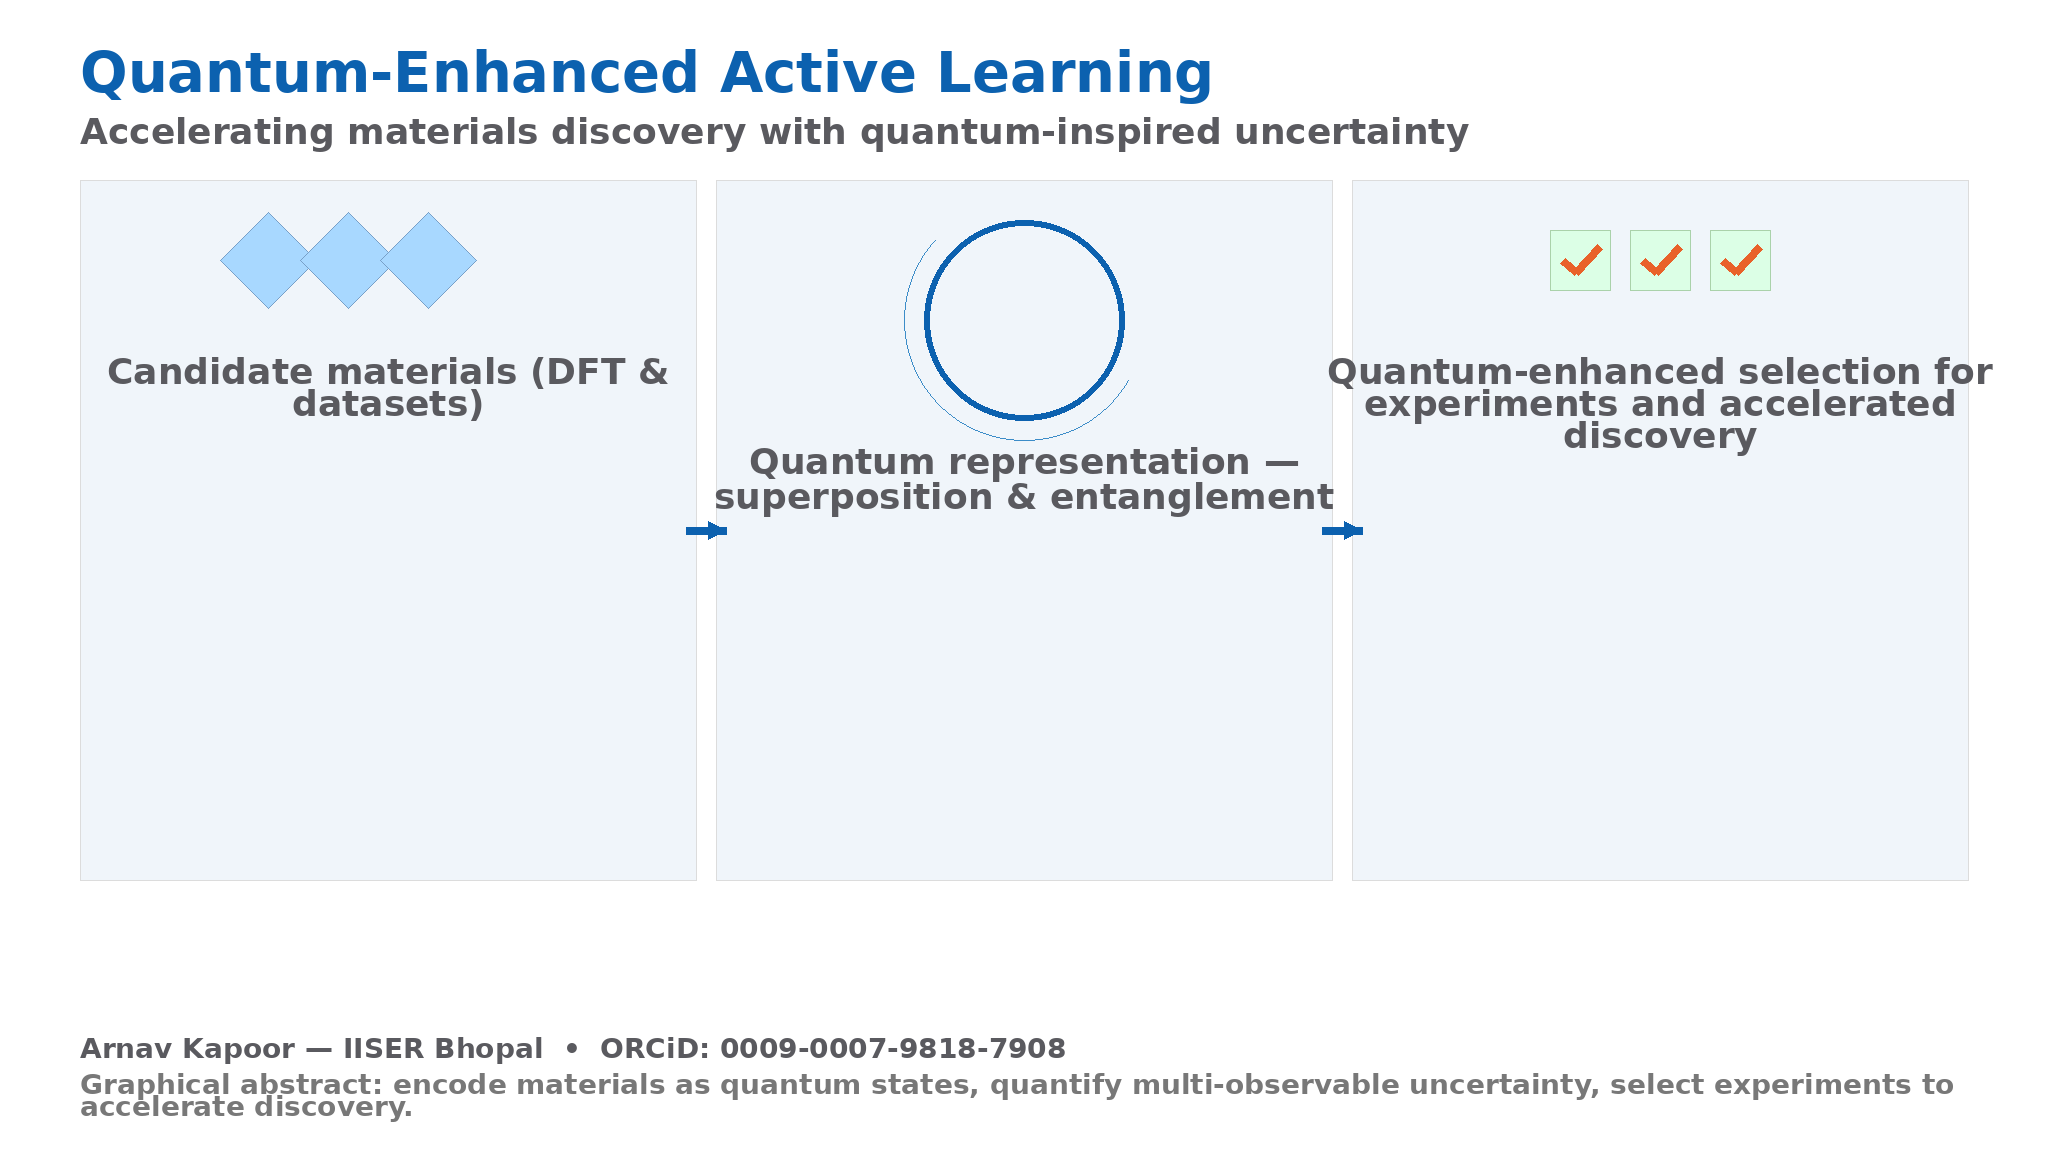
\includegraphics[width=0.8\textwidth]{graphical_abstract.png}
\caption{Method schematic: feature encoding, observables, and selection score computation.}
\label{fig:schematic}
\end{figure}

\section*{Experimental protocol}
We evaluate on two regression tasks (band gap, formation energy) using realistic features. Protocol: 5 independent trials, 70\% pool / 30\% held-out test, initial labeled set of 50, 8 iterations of batch selection (b=15). Baselines include Query-by-Committee, Expected Improvement, BADGE, CoreSet, uncertainty sampling, and random sampling. Metrics: test $R^2$, sample efficiency (iterations to reach a performance threshold), and paired t-tests.

\section*{Results}
The quantum-inspired method attains the highest mean test $R^2$ across both tasks (Table and detailed numbers in the repository). Learning curves (Figure~\ref{fig:learning}) show faster convergence and reduced variance across trials. Ablations indicate cross-observable covariance terms materially contribute to sample-efficiency gains.

\begin{figure}[ht]
\centering
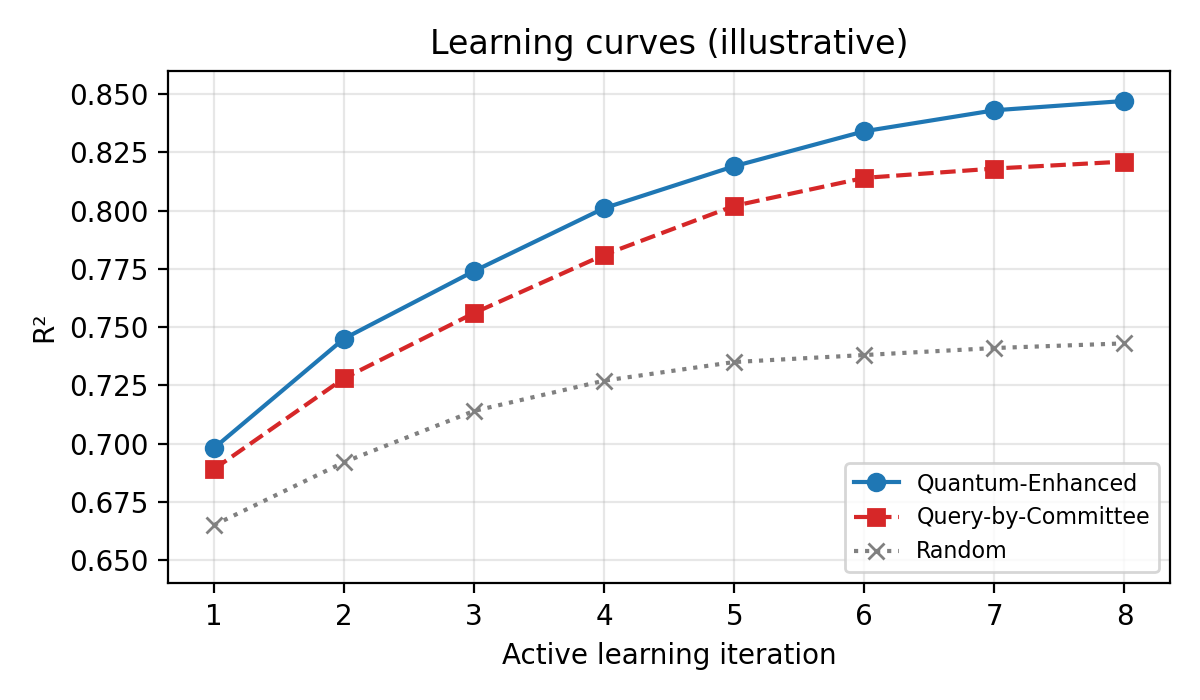
\includegraphics[width=0.8\textwidth]{fig2_learning_curve.png}
\caption{Illustrative learning curves (R² vs iteration) comparing the proposed method to strong baselines.}
\label{fig:learning}
\end{figure}

\section*{Conclusions and impact}
Aggregating multi-observable variance and covariance via quantum-inspired encodings yields a practical, model-agnostic selection strategy that improves sample efficiency in materials discovery. The approach is compatible with self-driving laboratory workflows and can be extended to multi-objective selection or integrated with experimental cost models. All code and preprocessing scripts are released to enable reproduction.

\vspace{6pt}
\noindent\textbf{Keywords:} quantum-inspired; active learning; uncertainty quantification; materials discovery; sample efficiency

\end{document}
